\subsection{Kiuwan}
Kiuwan was used for static analysis of PHP code for finding vulnerablities in the application.
\subsubsection{InternetBanking}
InternetBanking showed 2266 defects, out of which 76 were of high priority. Refer \ref{fig:kiuwan_overview}. The tool reported issues in the following categories:
\begin{itemize}
    \item Security
    \item Efficiency
    \item Reliability
    \item Portability
    \item Maintainability
\end{itemize}
We analyzed the issues in the Security category and found some false positives. However, few issues turned out to be actual bugs.
\begin{itemize}
	\item \textbf{Use of weak cryptographic hash} The user passwords are encrypted using \code{md5} before storing in the database. Since \code{MD5} has several weaknesses when used to generate cryptographic hashes, this is a serious vulnerability. This has been discussed in more detail in section \ref{OTG-AUTHN-007}. See \ref{fig:kiuwan_weak_hash} for the Kiuwan report.
	\item \textbf{Use of hardcoded password} The database credentials are stored in the file \code{DataAccess.php}. Also, these values are not defined at one place and used throughout code. Rather, the same hard-coded credentials can be found in several functions in the entire file. See \ref{fig:kiuwan_hardcoded_password} for the Kiuwan report.
	\item \textbf{Improper neutralization of input during web content generation (XSS)} It was found that it is possible to perform XSS attacks from the \code{Make Payment} interface. However, since it does not affect any functionality or other users, it could be considered low in priority. Refer \ref{OTG-INPVAL-001} for more detail. See \ref{fig:kiuwan_xss} for the Kiuwan report.
\end{itemize}

\subsubsection{SecureBank}
SecureBank showed 3010 defects, out of which 18 were of high priority. Refer \ref{fig:kiuwan_overview_secure_bank}. The tool reported issues in the following categories:
\begin{itemize}
    \item Security
    \item Efficiency
    \item Reliability
    \item Portability
    \item Maintainability
\end{itemize}
We analyzed the issues in the Security category and found that all of them were false positives which was also confirmed by black box testing and manual code inspection.

\begin{figure}[ht]
	\centering
	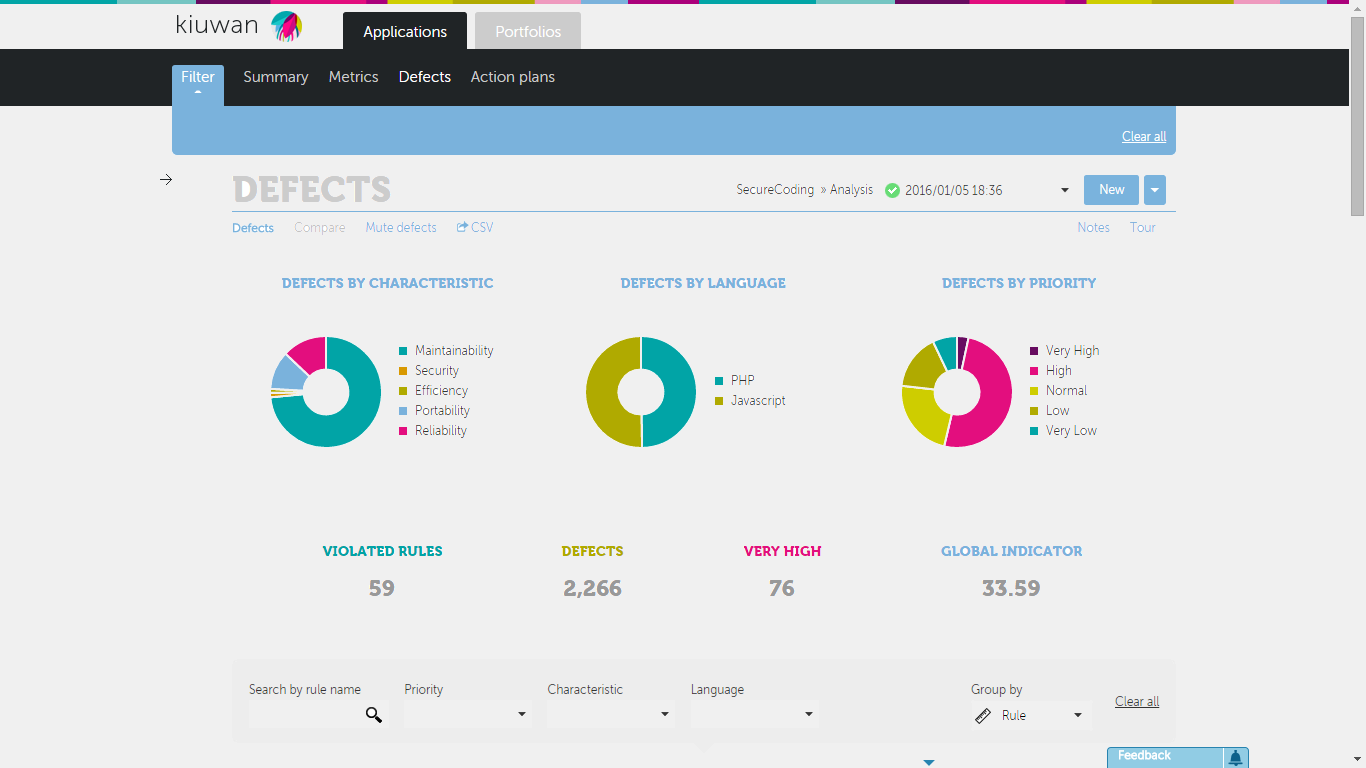
\includegraphics[width=.8\linewidth]{figures/kiuwan_overview.png}
	\caption{Overview of Kiuwan scan for InternetBanking}
	\label{fig:kiuwan_overview}
\end{figure}

\begin{figure}[ht]
	\centering
	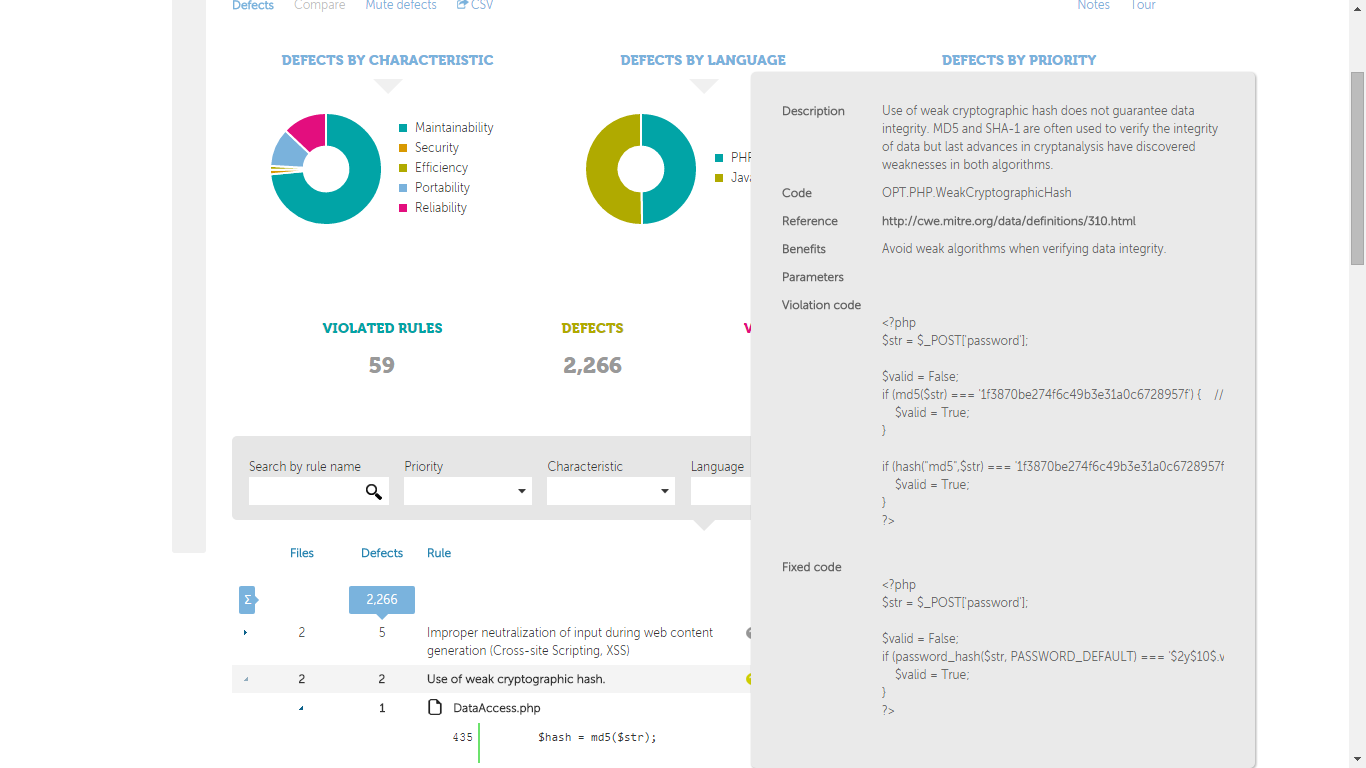
\includegraphics[width=.8\linewidth]{figures/kiuwan_weak_hash.png}
	\caption{Kiuwan: Weak Cryptographic hash vulnerability reported for InternetBanking}
	\label{fig:kiuwan_weak_hash}
\end{figure}

\begin{figure}[ht]
	\centering
	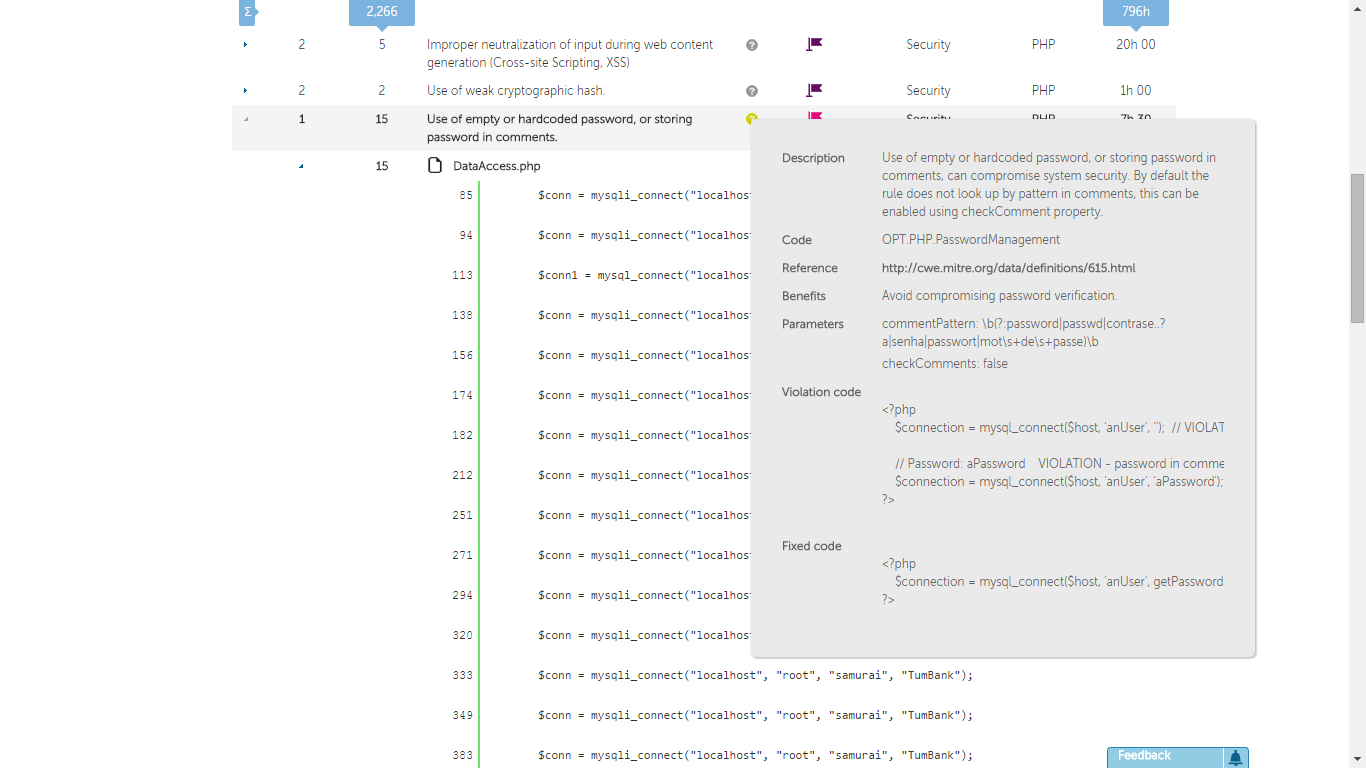
\includegraphics[width=.8\linewidth]{figures/kiuwan_hardcoded_password.png}
	\caption{Kiuwan: Hardcoded Password vulnerability reported for InternetBanking}
	\label{fig:kiuwan_hardcoded_password}
\end{figure}

\begin{figure}[ht]
	\centering
	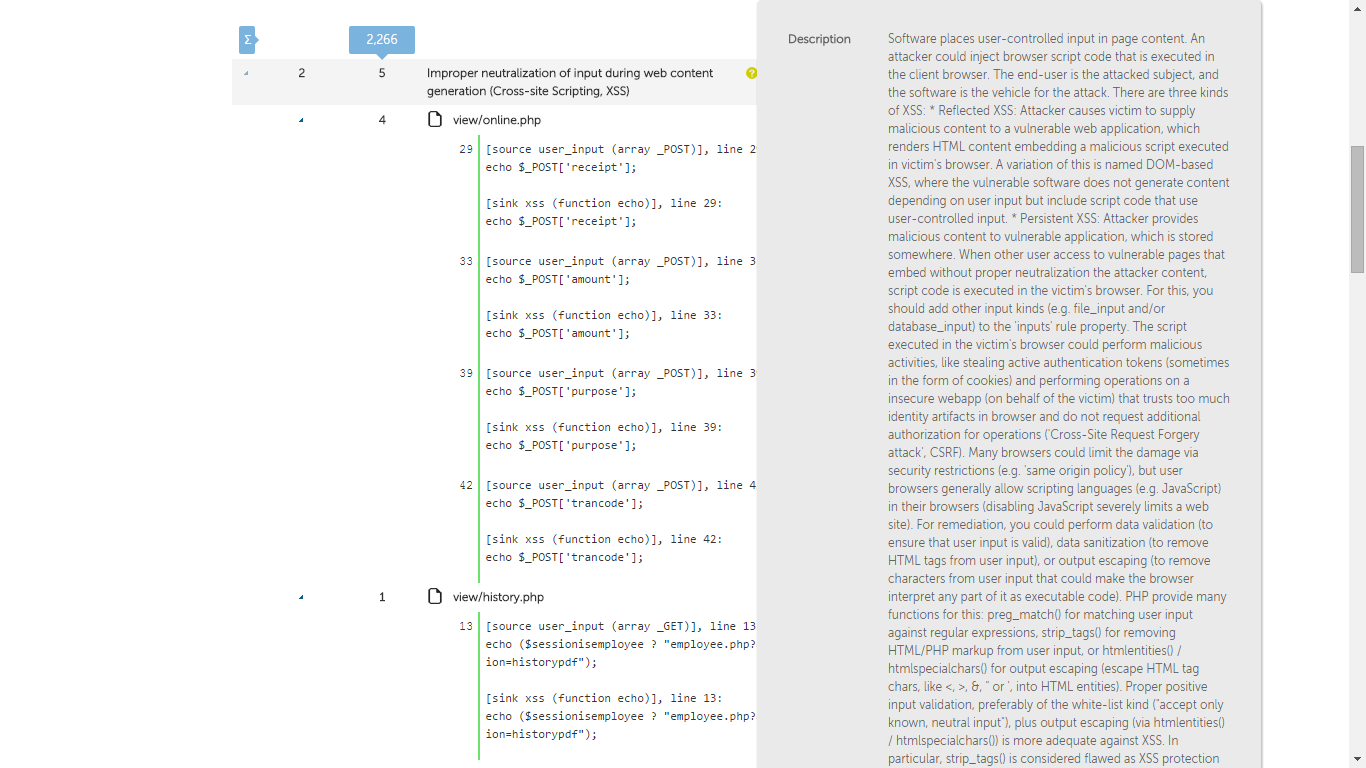
\includegraphics[width=.8\linewidth]{figures/kiuwan_xss.png}
	\caption{Kiuwan: XSS vulnerability reported for InternetBanking}
	\label{fig:kiuwan_xss}
\end{figure}

\begin{figure}[ht]
	\centering
	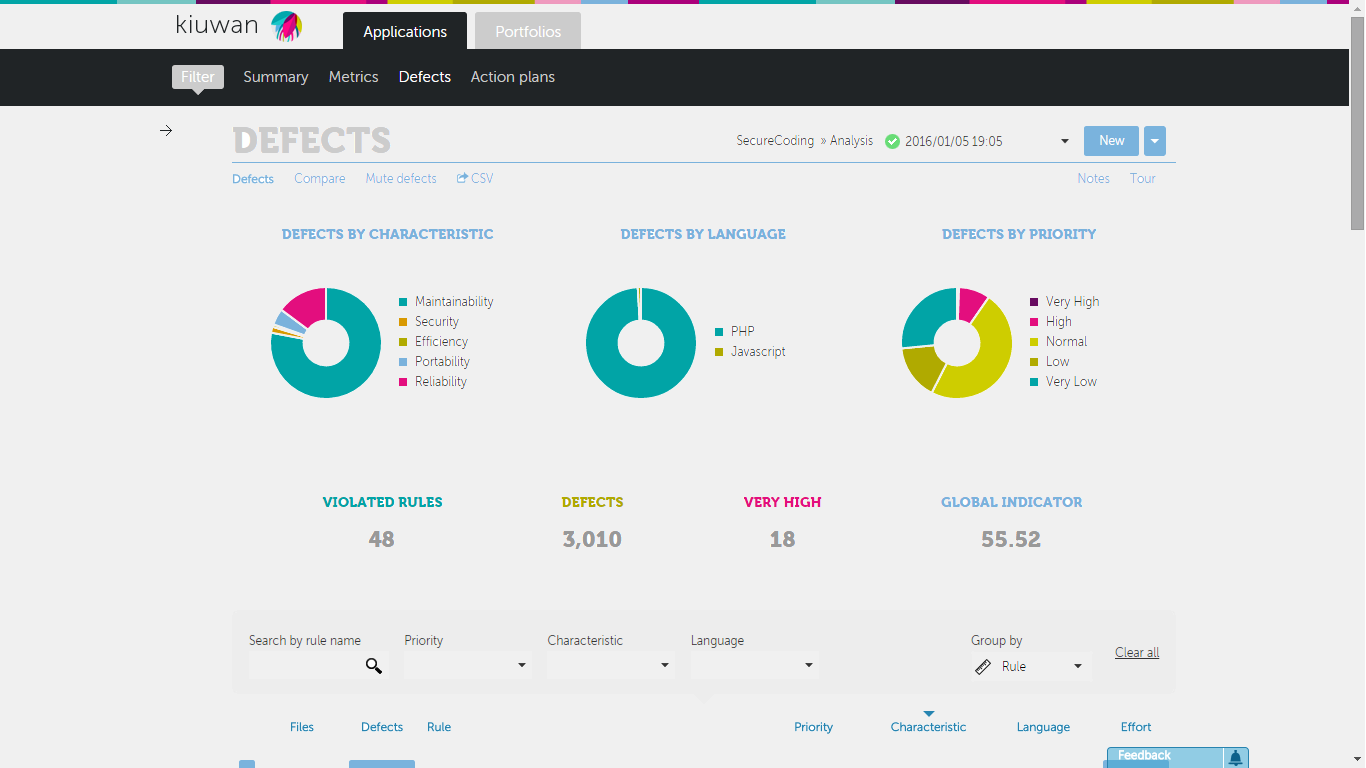
\includegraphics[width=.8\linewidth]{figures/kiuwan_overview_secure_bank.png}
	\caption{Overview of Kiuwan scan for SecureBank}
	\label{fig:kiuwan_overview_secure_bank}
\end{figure}